\newpage
\section{Conception du projet}
\label{sec:concept}

\noindent Cette section explicitera nos différentes idées de conceptions sur plusieurs points clés du projet, tel que l'IHM Graphique ou encore le moteur, pour répondre aux différentes spécifications énonces en \ref{sec:specification}.

\subsection{Conception Algorithmique}

\paragraph{}
    Cette sous-section est dédiée aux ébauches d'idées de conception concernant toute la partie algorithmique du projet tel que le système d'action, les déplacements ou la réflexion autour des classes de données.

\subsubsection{Classe de donnée}
\label{sec:donnee}

\paragraph{}
    La réflexion autour des classes de données est importante pour la conception d'un logiciel. En effet, ce fut la première étape de la réflexion autour de notre projet et elle a orienter la totalité de notre conception algorithmique.

\paragraph{}
    Pour commencer, nous allons présenter sous forme de diagramme de classe nos principales classes de données puis expliquer la réflexion qui en découle.

\begin{figure}[h]
\centering
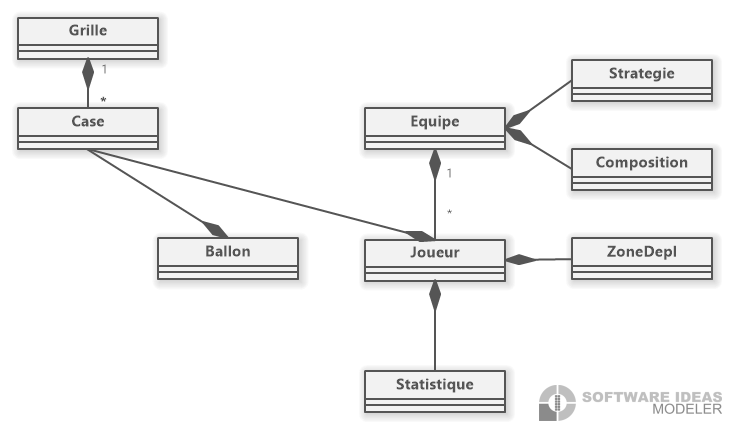
\includegraphics[width=17cm,height=15cm]{images/Classdiagram.png}
\caption{Classe de donnée}
\label{fig:classDonnee}
\end{figure}

\paragraph{}
    Comme on peut l'apercevoir sur \ref{fig:classDonnee}, une classe de donnée semble être la classe principale, c'est la classe Equipe. En effet, cela correspond a la réflexion que nous avons eux en début de projet, celle de se concentrer sur les blocs équipes avant de rentrer dans les réflexions individuelles.
\paragraph{}
    Aussi, a partir de \ref{fig:classDonnee}, on remarque la présence de statistiques unique a chaque joueur, le fait que les positions soient gérer par une grille et enfin la gestion des joueurs, de la stratégie et la composition est donnée à la classe Equipe.
    

\subsubsection{Systèmes de Manager}
\label{sec:managers}

\paragraph{}
    Dans cette section, nous détaillerons les différentes idées de conception autour de la gestion d'action et de déplacements.

\begin{table}[h!]
    \centering
    \begin{tabular}{|c|c|}
    \hline
    Nom Classe & Fonction\\
    \hline
    ManagBall & Gestion de toutes les actions autour du ballon\\
    \hline
    ManagDepl & Gestion de tous les deplacements de notre simulation\\
    \hline
    Manager & Classe qui permet la transmission et l'interaction entre les deux managers\\
    \hline
    \end{tabular}
    \caption{Répartition des taches entre les managers}
    \label{tab:managers}
\end{table}

\paragraph{Gestion des actions: }
    Comme expliquer dans \ref{tab:managers},la gestion des actions a été regrouper dans une seule et même classe : ManagBall. A l'intérieur de cette classe, les actions sont créer et peuvent interagir entre elles, par exemple, la possibilités de pouvoir intercepter la balle pendant une passe. C'est pour cela que nous avions décider de bien séparer la gestion des actions.

\paragraph{Gestion des déplacements: }
    Comme expliquer dans \ref{tab:managers},la gestion des deplacements a été regrouper dans une seule et même classe : ManagDepl. Comme expliquer dans \ref{sec:donnee}, la réflexion de toute la simulation est en priorité porter à l'équipe. Lors de la conception, nous avons imaginer le fonctionnement des déplacements de tel sorte que, d'abord, le bloc équipe monte ou descende en fonction de la possession ou non du ballon, puis seulement, un mouvement individuel des joueurs.
\newpage
\subsection{Conception IHM Graphique}
\label{sec:conceptGraph}

\paragraph{}
    Cette sous-section est dédiée aux ébauches d'idées de conception concernant toute la partie graphique du projet.
    
\begin{figure}[h]
\centering
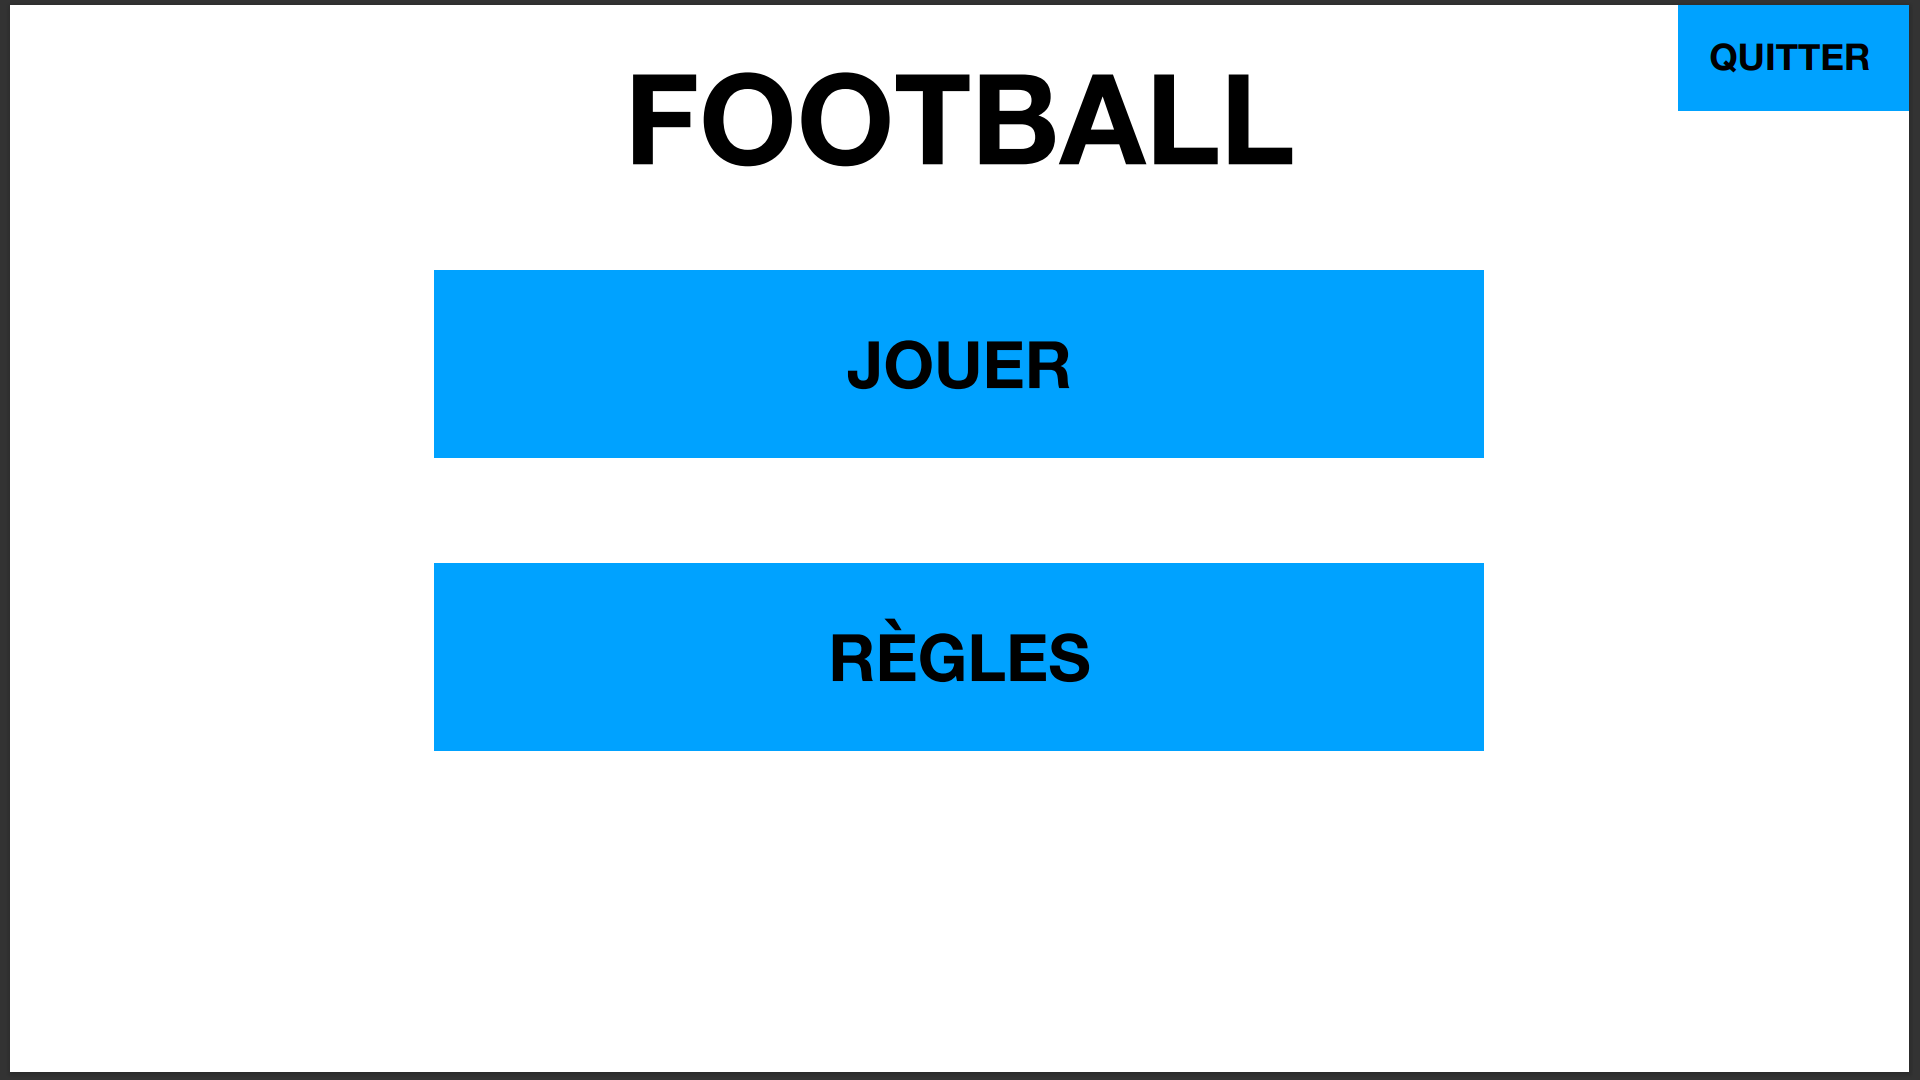
\includegraphics[width=12.82cm, height=8.2cm]{images/ConceptIHM1.png}
\caption{Conception page d'accueil}
\label{fig:accueil}
\end{figure}

\paragraph{Conception de la page d'accueil}
    Pour notre page d'entrée, notre première idée était de concevoir une page d'accueil basique que l'on peut voir dans n'importe quel jeu vidéo. 
    
    \vspace{15pt}

\begin{itemize}
    \item \textbf{Jouer :} 
        Si vous appuyez sur le bouton "Jouer" situé en haut, vous serez redirigé vers la page suivante qui vous permettra de choisir votre équipe.

    \vspace{15pt}

    \item \textbf{Règles :} 
        Si vous appuyez sur le bouton "Règles" situé au milieu, cela vous amènera sur la page des règles du jeu de football.

    \vspace{15pt}

    \item \textbf{Quitter :} 
        Si vous appuyez sur le bouton "Quitter" situé en bas, cela vous permettra de quitter le jeu.
        
    \vspace{15pt}
\end{itemize}

\newpage

\begin{figure}[h]
\centering
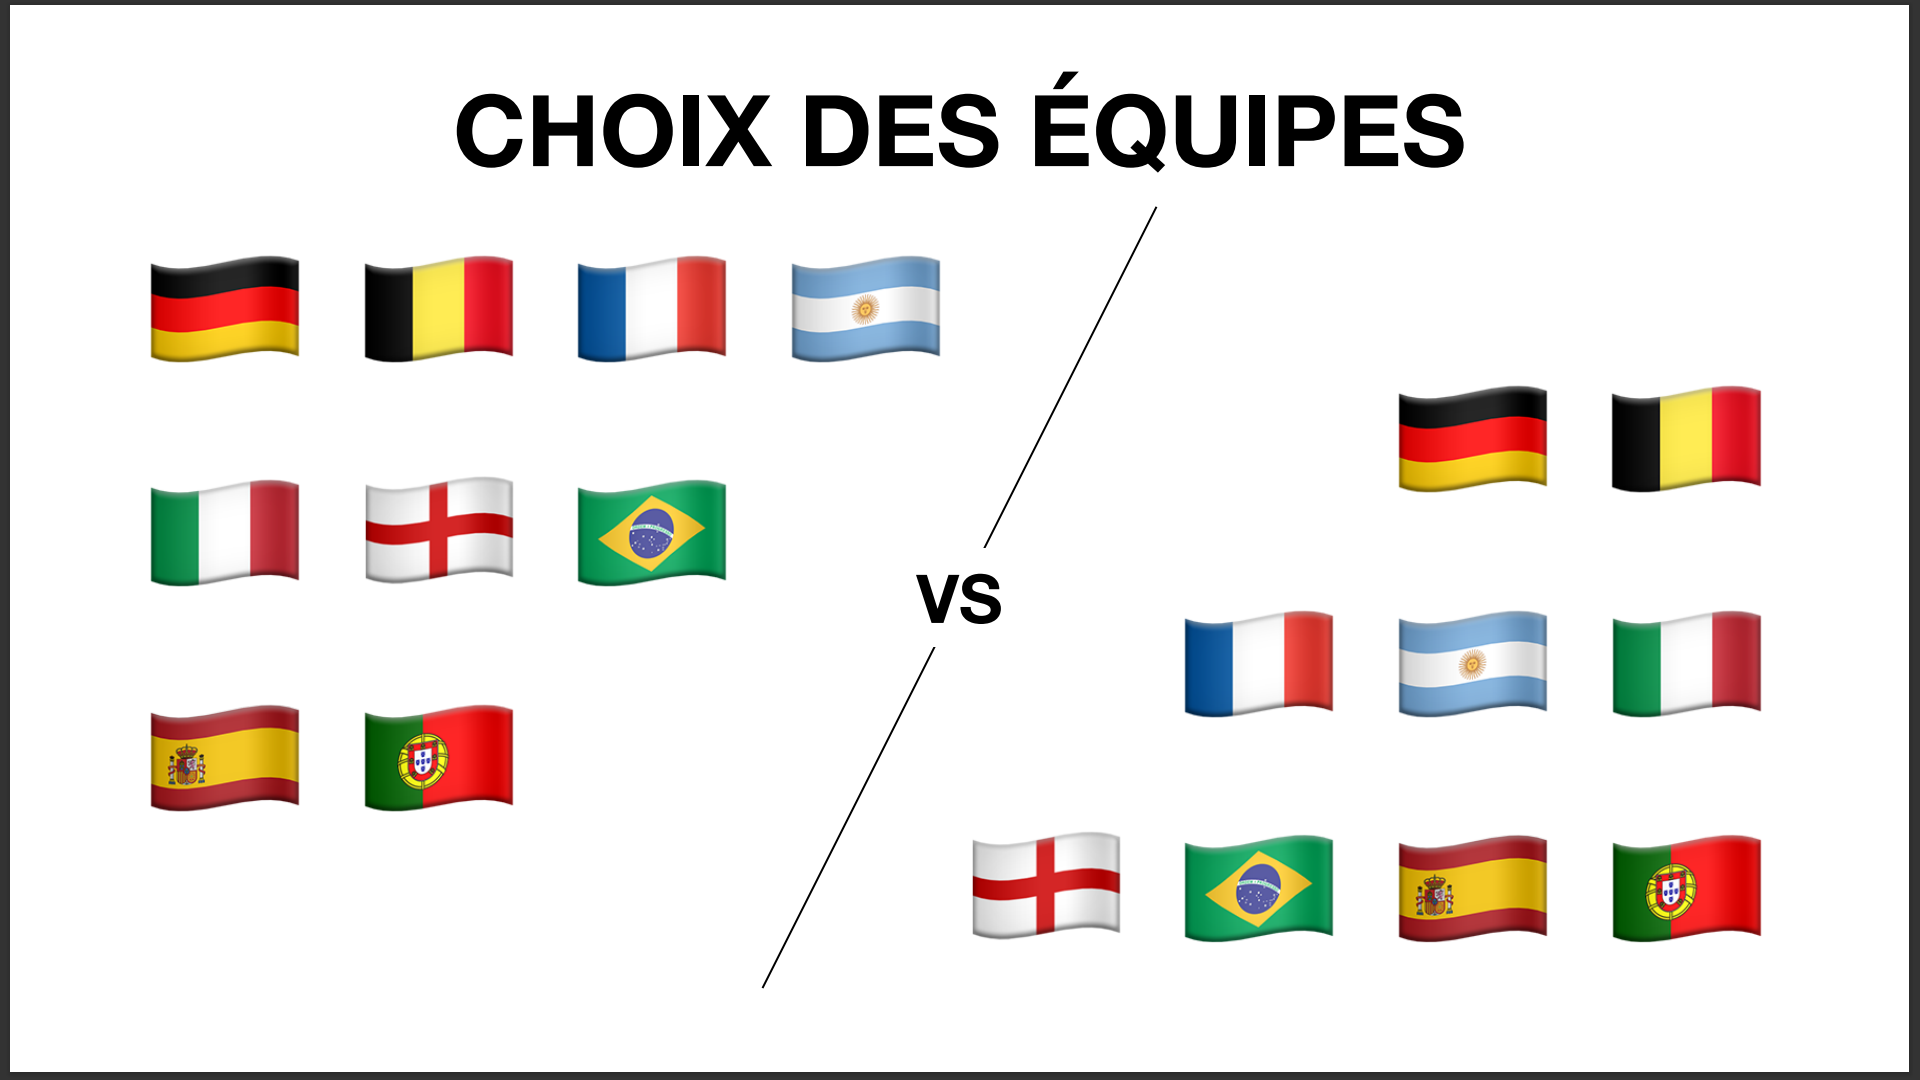
\includegraphics[width=12.82cm, height=8.2cm]{images/ConceptIHM2.png}
\caption{Conception Choix Equipe}
\label{fig:choixEquipe}
\end{figure}

\paragraph{Conception de la page du choix des équipes}
    On avait pour concept de permettre aux utilisateurs de choisir le pays que leur équipe représentera afin de leur donner le sentiment de maîtriser leur équipe et de leur permettre de choisir leur adversaire avant le match. Cette page est accessible depuis la page d'accueil lorsque le joueur clique sur le bouton "Jouer".

\vspace{15pt}
    
\begin{itemize}
    \item \textbf{Les équipes :} 
        Au milieu de l'écran, vous pouvez voir des drapeaux de pays parmi lesquels l'utilisateur pourra choisir celui qui représentera son équipe ainsi que celui de l'équipe adverse.
        
    \vspace{15pt}
\end{itemize}

\begin{figure}[h]
\centering
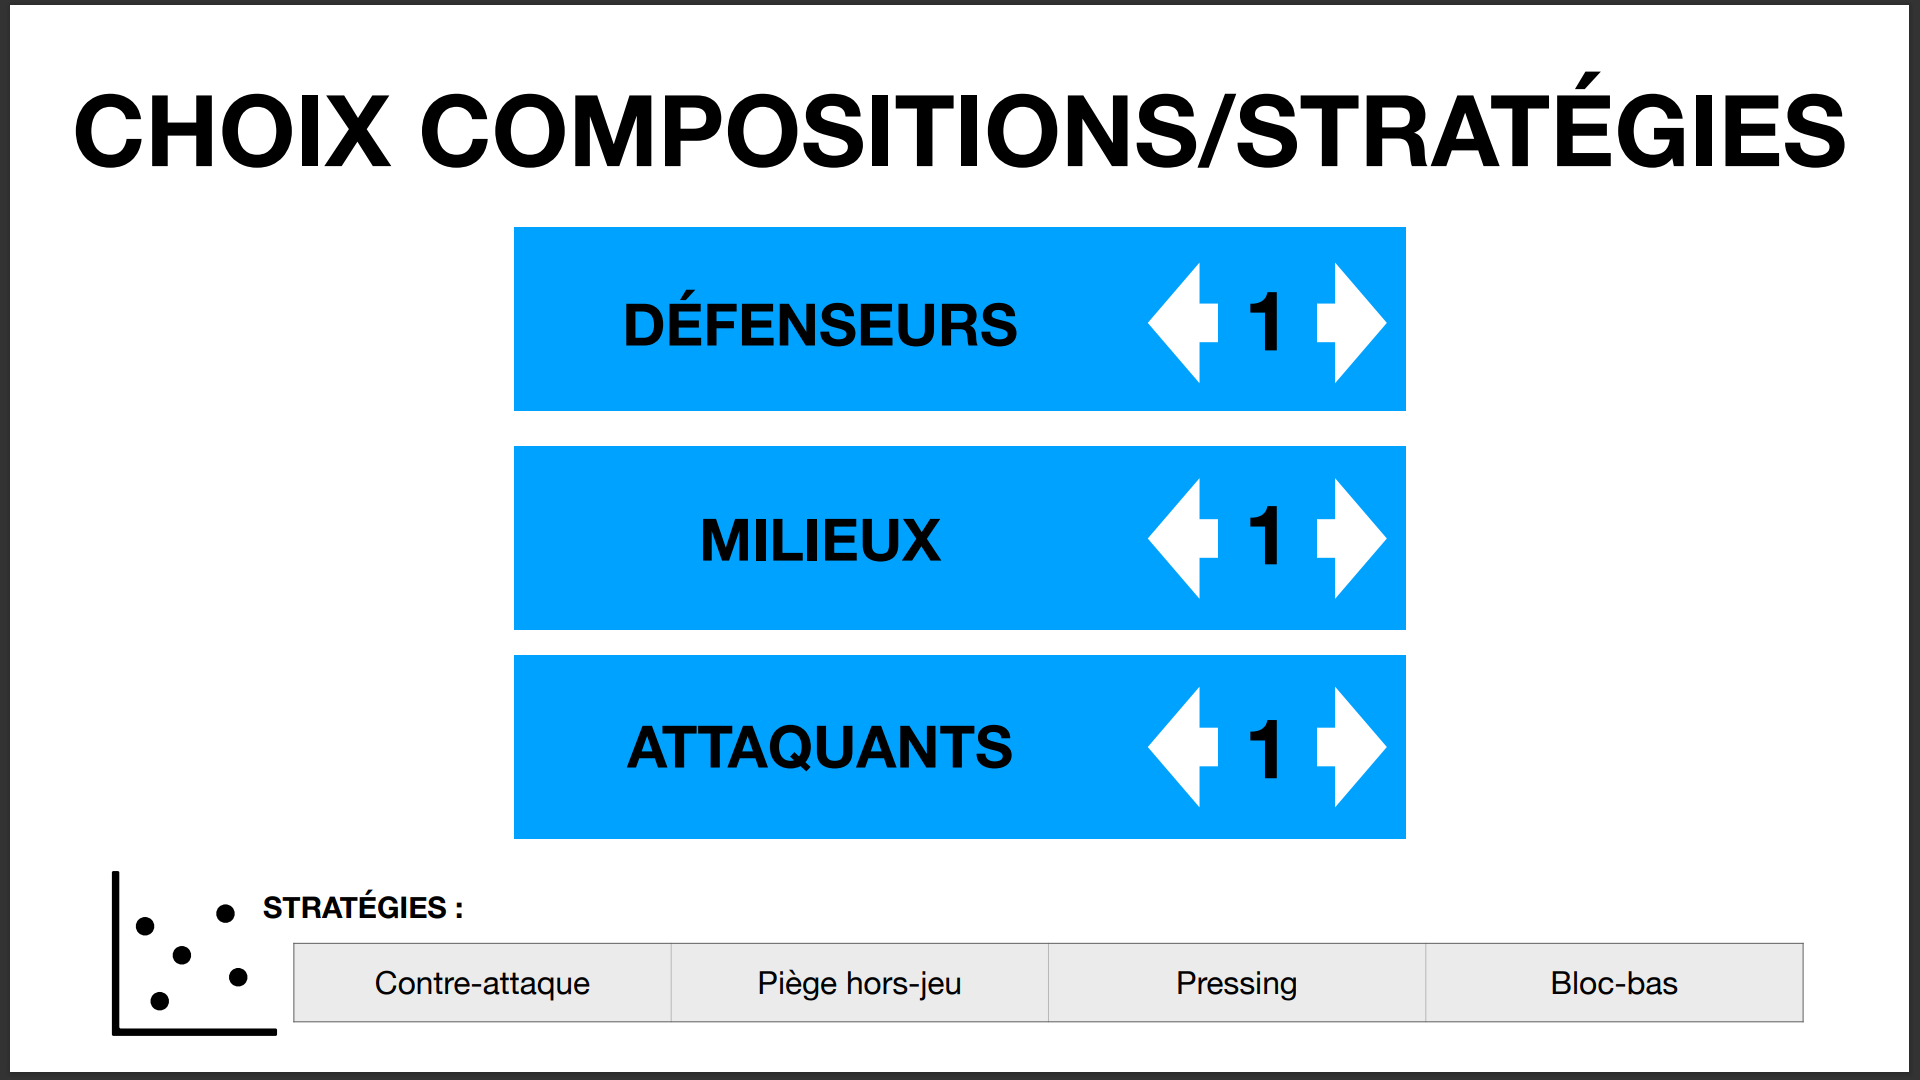
\includegraphics[width=12.82cm, height=8.2cm]{images/ConceptIHM3.png}
\caption{Conception Choix Poste}
\label{fig:choixPoste}
\end{figure}

    \vspace{15pt}
    \vspace{15pt}

\paragraph{Conception de la page de la sélection de votre composition}
    Cette page est l'une des plus importantes, car elle permet à l'utilisateur de choisir la composition de son équipe. Nous tenions vraiment à ce que l'utilisateur se sente maître de son équipe, c'est pourquoi nous lui donnons la possibilité de choisir sa formation. En ce qui concerne la stratégie, nous avons décidé de l'enlever, car nous avons jugé que son développement algorithmique serait trop compliqué à réaliser dans le temps imparti. Cette page fait suite à la page Choix des Équipes.

    \vspace{15pt}

\begin{itemize}
    \item \textbf{Les postes :} 
        Au milieu de votre écran, vous pouvez voir les différents postes avec deux flèches une vers la droite et l'autre vers la gauche, ainsi qu'un chiffre au milieu qui indique le nombre de joueurs sur chaque poste. Les flèches permettent d'ajouter ou de retirer un joueur à chaque poste.
    \vspace{15pt}
\end{itemize}

\begin{figure}[h]
\centering
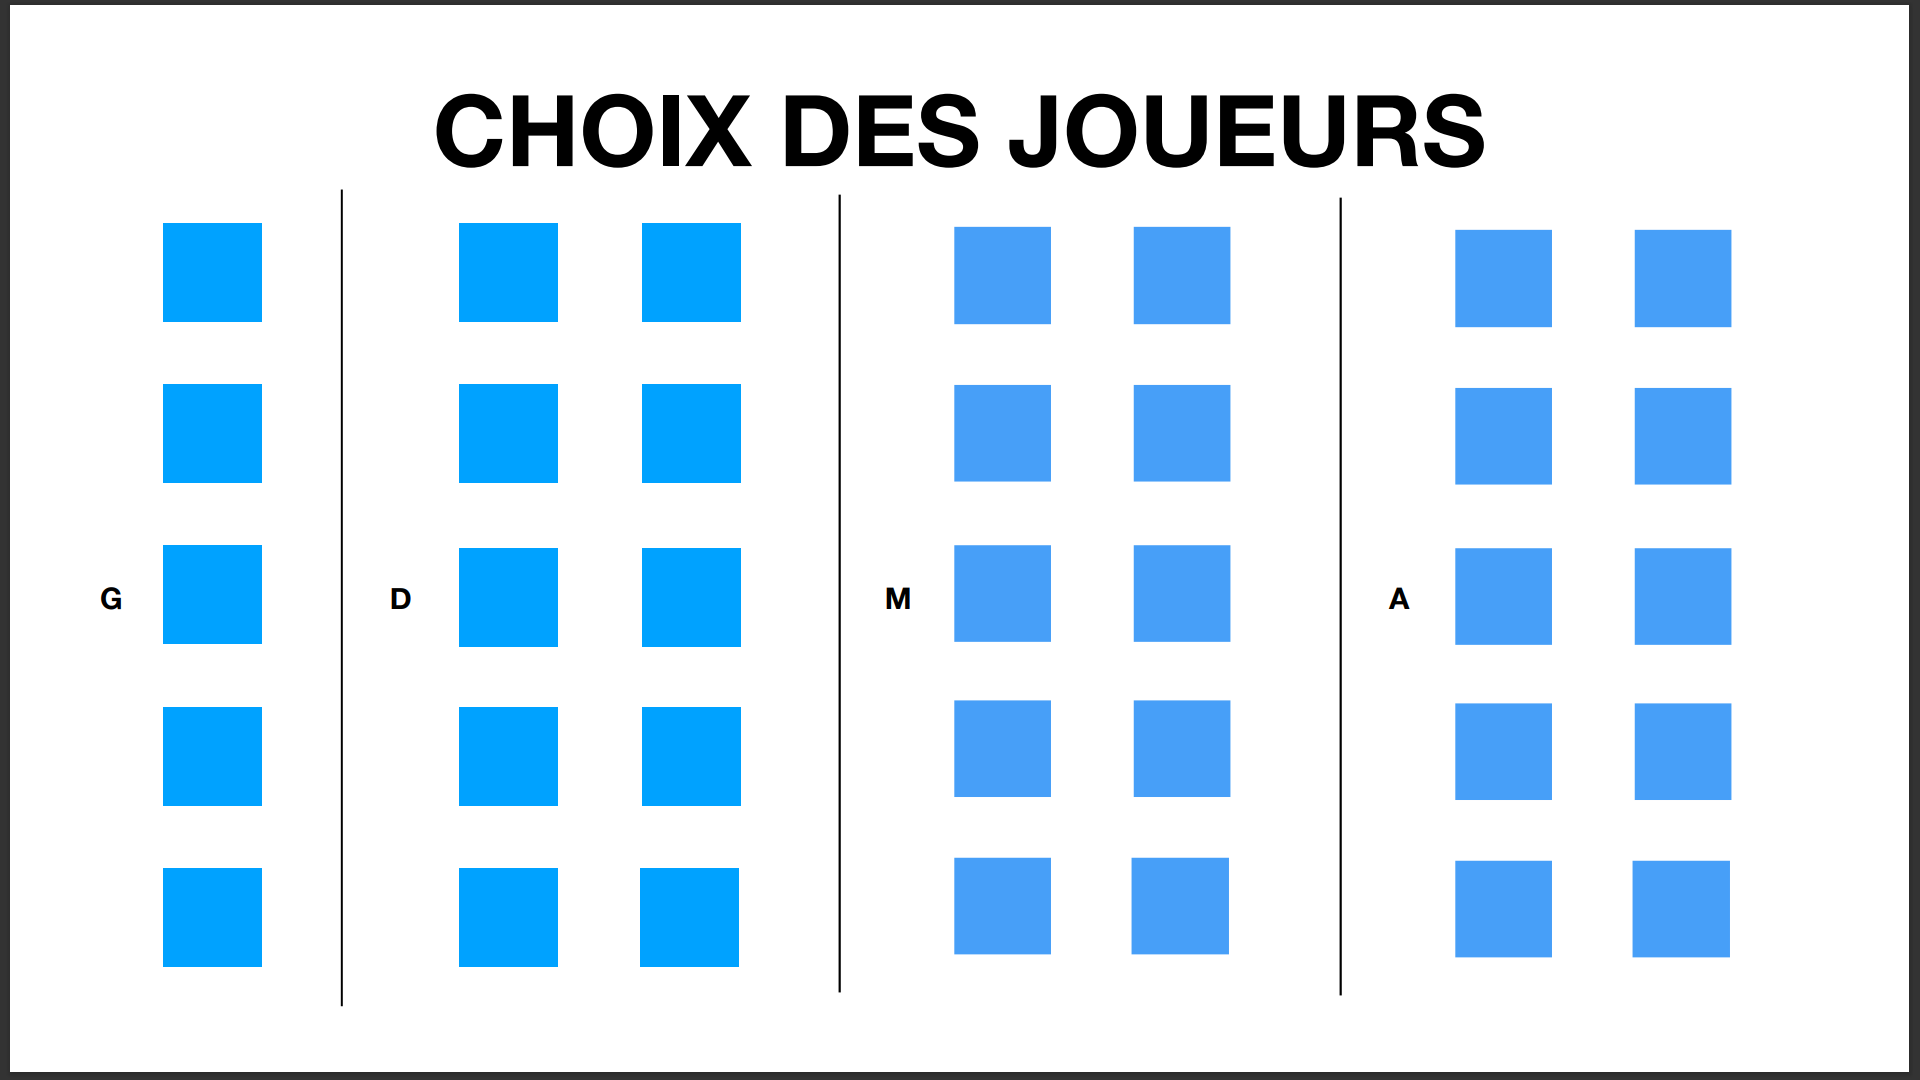
\includegraphics[width=12.82cm, height=8.2cm]{images/ConceptIHM4.png}
\caption{Conception Choix Joueur}
\label{fig:choixJoueur}
\end{figure}

    \vspace{15pt}

\paragraph{Conception de la page de la sélection de vos joueurs}
    Cette page est l'une des pages les plus importantes puisque elle permet à l'utilisateur de choisir les joueurs qui composeront son équipe. Nous avons décidé de laisser à l'utilisateur la possibilité de choisir les joueurs pour qu'il puisse prendre les meilleurs joueurs disponibles et ainsi être le chef d'orchestre de son équipe. Cette page fait suite à la page Choix de Postes.

    \vspace{15pt}

\begin{itemize}
    \item \textbf{Les joueurs :} 
         Au milieu de l'écran, l'utilisateur peut sélectionner les joueurs pour chaque poste en cliquant sur le chiffre correspondant. Par exemple, s'il a choisi d'avoir trois attaquants dans la page précédente, il peut sélectionner 3 attaquants en cliquant sur les joueurs à côté de "A". Il peut faire de même pour le gardien "G", les défenseurs "D" et les milieux "M".
    \vspace{15pt}
\end{itemize}

\newpage

\begin{figure}[h]
\centering
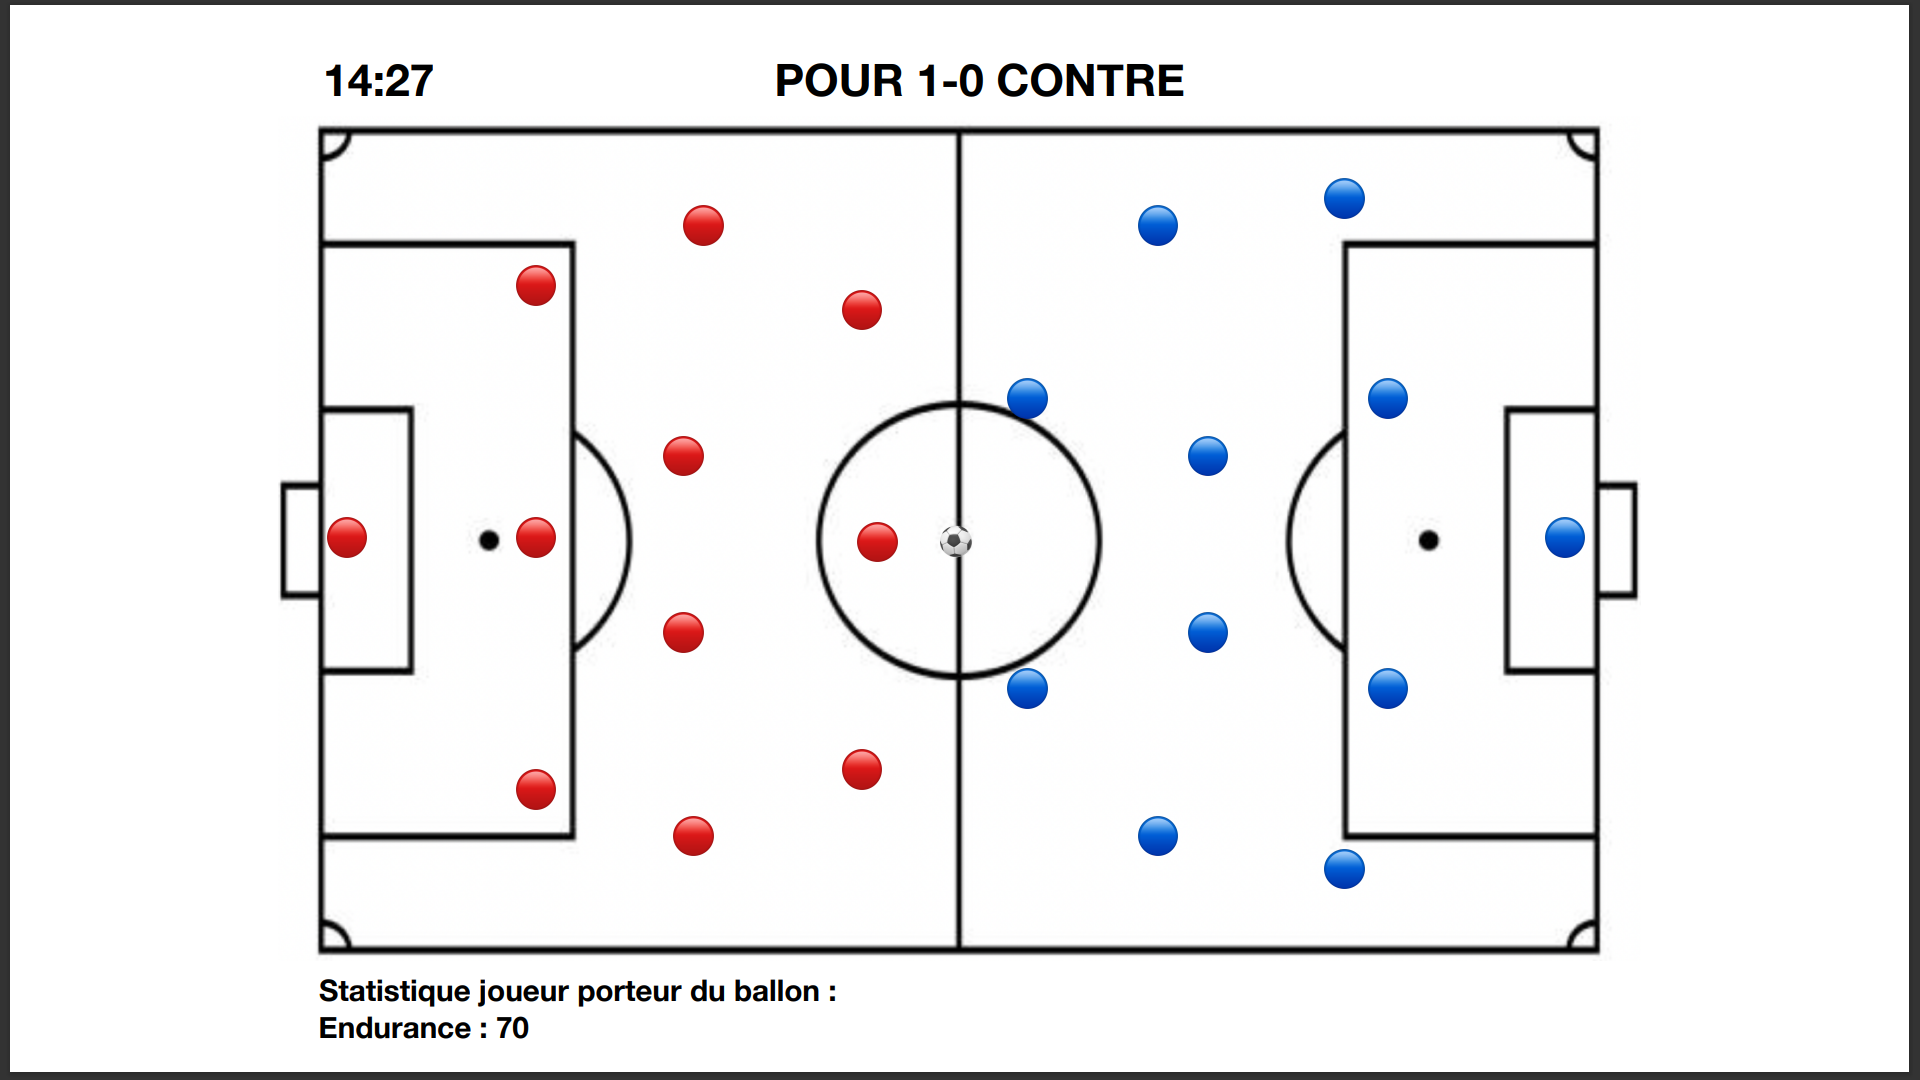
\includegraphics[width=12.82cm, height=8.2cm]{images/ConceptIHM5.png}
\caption{Conception de la simulation }
\label{fig:match}
\end{figure}

    \vspace{15pt}
\paragraph{Conception de la page de la simulation du match}
    C'est la page principale de notre simulation, car c'est lors du match que tous les choix de l'utilisateur vont s'impliquer. Nous avons voulu rester fidèles à l'expérience d'un match de football en permettant à l'utilisateur de voir le score et le temps. Nous avons décidé de ne pas afficher le joueur ayant la balle, car nous ne l'avons pas jugé pertinent. Cette page est la suite de la page Choix des Joueurs.

\vspace{15pt}

\begin{itemize}
    \item \textbf{Temps :} 
        Le chronomètre est indiqué à gauche des scores pour vous permettre de savoir combien de temps il reste avant la fin du match.

    \vspace{15pt}

    \item \textbf{Score :} 
         Le score est affiché juste au dessus du terrain. Ainsi, si l'équipe de l'utilisateur marque, il pourra le voir directement à cet endroit.

    \vspace{15pt}
            
    \item \textbf{Statistique du joueur ayant la balle :}
        La base de notre idée était de permettre à l'utilisateur de voir les statistiques du joueur ayant la balle en dessous du terrain, mais nous avons décidé de l'enlever comme cela a été expliqué précédemment.
    
    \vspace{15pt}
\end{itemize}

\newpage

\begin{figure}[h]
\centering
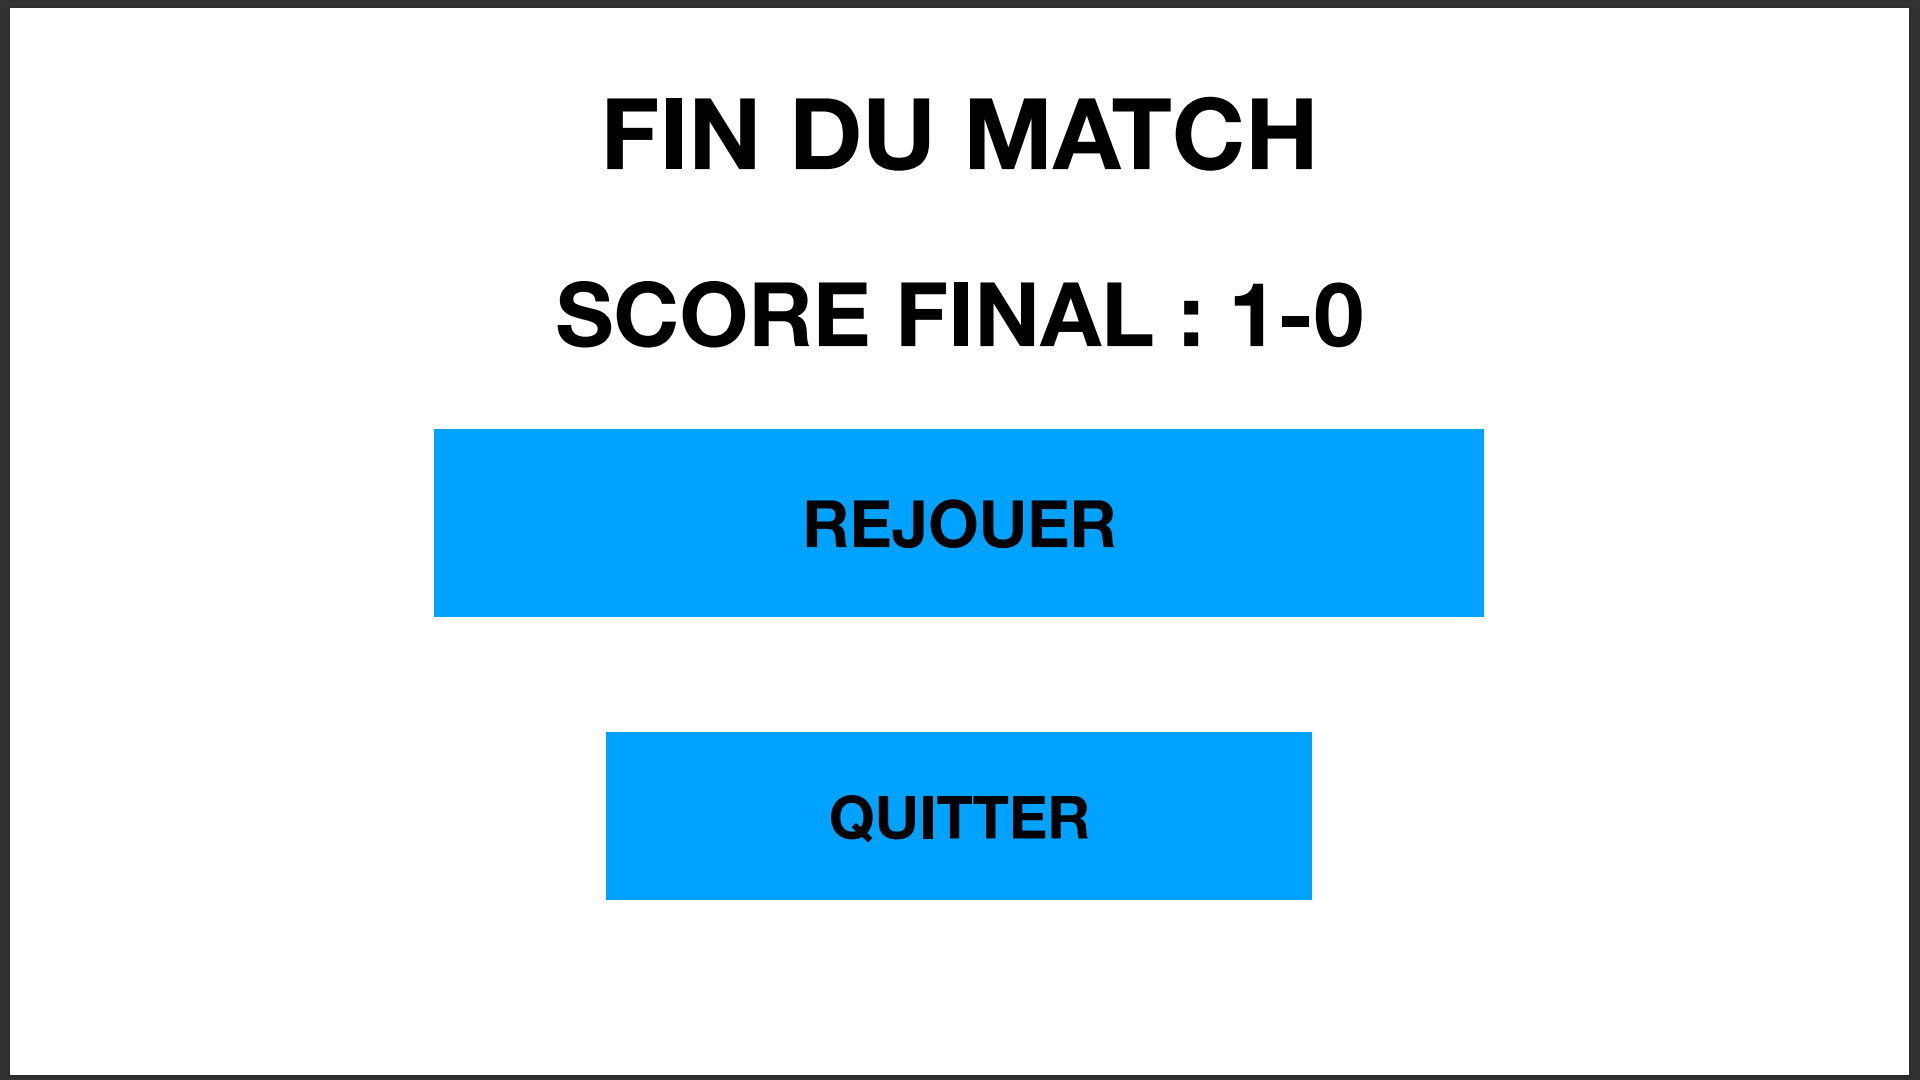
\includegraphics[width=12.82cm, height=8.2cm]{images/ConceptIHM6.png}
\caption{Conception Après Match}
\label{fig:stats}
\end{figure}

\vspace{15pt}

\paragraph{Conception de la page d'après match}
    Cette page est la dernière page après avoir fini le match. Elle permet la redirection vers la page d'entrée.

\vspace{15pt}
    
\begin{itemize}
    \item \textbf{Rejouer :} 
        Si vous appuyez sur le bouton "Rejouer", vous serez redirigé directement vers la page du choix des équipes.

    \vspace{15pt}

    \item \textbf{Quitter} 
         Si vous appuyez sur le bouton "Quitter", cela vous fera quitter la simulation.

    \vspace{15pt}
            
    \item \textbf{Le score :}
        Le score situé au-dessus du bouton "Rejouer" est le score de fin de match.
        
    \vspace{15pt}
\end{itemize}